% Picar el capitulo entre Implementacion y Experimentos
% Añadir un p\'arrafo al final de Implementacion de como se utilza el nuevo sistema
\chapter{Implementación}\label{chapter:implementation}
En este cap\'itulo se muestra una implmentaci\'on la propuesta utilizando a AutoGOAL (\cite{estevez2020solving}) como sistema de AutoML. AutoGOAL utliza programaci\'on evolutiva para producir sus resultados, precisamente la  proceso es la se encuentra principalmente en contacto con nuestra propuesta, por tanto es importante antes de adentrarse en el proceso de implementaci\'on en s\'i entender la base te\'orica en la que se apoya AutoGOAL para modelar su espacio de b\'usqueda.

\section{Marco Te\'orico de AutoGOAL}

Nuestra implementaci\'on est\'a basada en AutoGOAL (\cite{estevez2020solving}) un sistema de AutoML que modela el espacio de decisi\'on basado una Gram\'atica Probabil\'istica  Libre del Contexto (\textit{Probabilistic Context Free Grammar}, PCFG) y utiliza Evoluci\'on Gram\'atica Probabil\'istica (\textit{Probabilistic Grammatic Evolution} para modelar dirigir el espacio de b\'usqueda. 

PCFG se define como una quinterna $PG = (NT, T, S, P, Prob)$ donde $NT$ y $T$ representan los conjuntos disjuntos no vac\'io de los s\'imbolos no terminales y terminales respectivamente. $S$ representa el No Terminal inicial con el que es posible expandir toda la gram\'atia. $P$ es el conjunto de reglas de producci\'on que rigen a la grma\'atica. $Prob$ (el elemento que hace que sea diferente que las gram\'aticas libres de contexto en general) es un conjunto de probabilidades asocaido con cada producci\'on de la gram\'atica. 

Para acutalizar el espacio de decisi\'on  se utiliza Evoluci\'on Gram\'atica Probabil\'istica (\textit{Probabilistic Grammatic Evolution}, PGE, \cite{megane2021probabilistic}), un algorimto de Estimaci\'on de Distribuci\'on (\textit{Estimation of Distribution ALgorithms, EDA}, \cite{larranaga2001estimation}) que remplaza los operadores cl\'asicos de mutaci\'on y cruce por un muestreado sobre las probabilidades de distribuci\'on de PCFG de acuerdo a las producciones utilizadas por el mejor individuo. 

\section{Implementaci\'on en AutoGOAL}

\begin{figure}[ht]
    \centering
    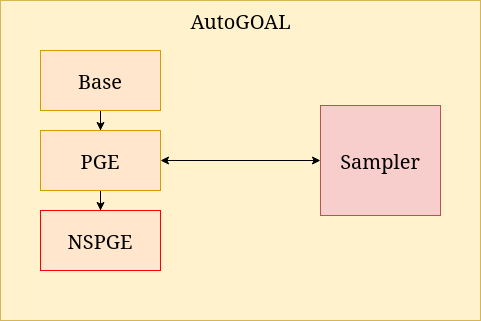
\includegraphics[scale=0.6]{Pictures/autogoal_impl.png}
    \caption{Diagrama general}
    \label{impl:fig:general_diagram}
\end{figure}


AutoGOAL es un sistema de AutoML gen\'etico que utiliza una Gram\'atica Probabil\'istica Libre del Contexto  para modelar su espacio de decisi\'on. Se representa utilizando un grafo aciclico dirigido (DAG) donde cada nodo de este representa una posible cadena de la gram\'atica y sus aristas apuntan a todas las posibles cadenas que se pueden generar a partir de estas sustituyendo alg\'un No Terminal por una producci\'on de la Gram\'atica. Cuando una cadena se encuentra completamente expandida, i.e. compuesta por solo simbolos terminales, se tiene una soluci\'on v\'alida del sistema. 

Inicialmente cada arista de este DAG se inicializa con una probabilidad igual a todas sus aristas hermanas (i.e. todas las aristas que salen de su mismo nodo) tal que la suma de sus probabilidades sea 1. Un camino se escoge utilizando una variable uniforme tal que su valor determina la arista a seleccionar. Cuando se tiene un individuo apto la manera de AutoGOAL de conservar sus ``genes'' es aplicando PGE sobre las aristas que conforman el camino que llevaron a esa soluci\'on. M\'as especificamente, la implementaci\'on de AutoGOAL de PGE dado $n$ individuos, son evaluados respecto a una funci\'on de evaluaci\'on $f$ y se crea una listas de las $k$ mejores soluciones (encabezada por la m\'as apta) y las aristas de las probabilidades se actualizan de acuerdo a estas soluciones. 

Se a\~nade a AutoGOAL la clase NSPGE, un m\'etodo de b\'usqueda inspirado en NSGA-II (\cite{deb2002fast}) que utiliza PGE como base. El objetivo de NSPGE es extender la funcionalidad de PGE para que sea capaz de seleccionar los $k$ mejores individuos de acuerdo a $m$ m\'etricas, con $m \ge 2$. La l\'ogica de la PGE encargada de ordenar los inidividuos m\'as aptos se encuentra en el m\'etodo \textit{\_inidices\_of\_the\_fittest\_} la cual NPSGE sobreescribe.

\subsection{NSPGE}

En NSPGE, dentro de \textit{\_inidices\_of\_the\_fittest\_} se aplica la ordenaci\'on definida por \cite{deb2002fast}. Dado $n$ soluciones se  agrupan seg\'un su \'indice de dominaci\'on (i.e. Non Dominated Sorting), donde cada agrupamiento se le llama frente de rango $i$, donde $i$ representa la cantidad de soluciones que dominan a cada una de estas. Una vez establecidos estos frentes se extraen las primeras $k$ soluciones, en caso de que no se pueda seleccionar un frente completo, se aplica Crowding Distance para seleccionar la muestra m\'as representativa de este.


\begin{lstlisting}[language=Python]
def _indices_of_fittest(self, fns: List[List[float]]):
  # Se ordenan todas las soluciones segun su orden
  # de dominacion
  fronts = self.non_dominated_sort(fns)
  indices = []
  k = int(self._selection * len(fns))

  for front in fronts:
    if len(indices) + len(front) <= k:
      indices.extend(front)
    else:
      # Cuando solo se utiliza una porcion del frente
      # se aplica crowding distance
      indices.extend(
          sorted(
              front,
              key=lambda i: -self.crowding_distance(fns, front, i)
          )[: k - len(indices)]
      )
      break
  return indices
\end{lstlisting}

\subsubsection{Non Dominated Sort}
La ordenaci\'on se conforma por dos pasos l\'ogicos fundamentales:
\begin{enumerate}
    \item Se verifica todo par de soluciones $x, y$ encontradas y se aplica $x \prec y$ con el objetivo de calcular el \'inidice de dominaci\'on de cada soluci\'on. Adem\'as se construye un DAG conformado por las soluciones donde existe una arista entre las soluciones $x$ y $y$ si $x \prec y$. La ra\'iz de dicho DAG est\'a conformado por las soluciones que nadie domina.
    \item Se recorre DAG utilizando una versi\'on de BFS ($Breadth First Search$) donde los soluciones visitadas se les reduce el \'indice de domianci\'on en uno. Si llega a 0 se a\~nade al frente de Pareto que se est\'a formando.
\end{enumerate}

\begin{lstlisting}[language=Python]
def non_dominated_sort(self, scores: List[List[float]]):
  # fronts almacena los frentes 
  #(i.e. fronts[i] es el frente de rango i)
  fronts: List[List[int]] = [[]]

  # domination_rank en i indica la cantidad de soluciones
  # que dominan a la solucion i
  domination_rank = [0] * len(scores)

  # dominated_scores en i alamacena las soluciones dominadas
  # por la solucion i
  dominated_scores = [list() for _ in scores]

  # revisa todo par de soluciones y se establece
  # quien dominan a quien
  for i, score_i in enumerate(scores):
    for j, score_j in enumerate(scores):
      if self._improves(score_i, score_j):
          dominated_scores[i].append(j)
      elif self._improves(score_j, score_i):
          domination_rank[i] += 1
    if domination_rank[i] == 0:
       fronts[0].append(i)

  # de acuerdo a la informacion sobre quienes
  # se dominan, forma todos los frentes
  front_rank = 0
  while len(fronts[front_rank]) > 0:
    next_front = []
    for i in fronts[front_rank]:
      for dominated in dominated_scores[i]:
        domination_rank[dominated] -= 1
        if domination_rank[dominated] == 0:
          next_front.append(dominated)
    front_rank += 1
    fronts.append(next_front)

  return fronts[:-1]
\end{lstlisting}

\subsubsection{Crowding Distance}
Se sigue la idea del algoritmo propuesto en (\ref{proposal:alg:cd}). Dado $m$ m\'etricas a evaluar se realizan $m$ iteraciones, donde en cada una se ordena alg\'un frente de rango $k$ de acuerdo a la metrica $m_i$. A la soluciones que con respecto a la m\'etrica $m_i$ tienen el m\'inimo y mayor valor se les asigna distancia infinita y luego se c\'alculan los valores intermedios. En \cite{deb2002fast} requiren que los valores de las m\'etricas esten normalizados, en nuestra implementaci\'on utilizamos \textit{feature scaling} para normalizar los valores entre 0 y 1.

\begin{lstlisting}[language=Python]
def crowding_distance(
    self, scores: List[List[float]], front: List[int], index: int
) -> float:
  # Crowding distance usa los vectores normalizados.
  # Se aplica feature scaling para llevar los vectores a [0, 1]
  scaled_scores = feature_scaling(scores)

  crowding_distances: List[float] = [0 for _ in scores]
  for m in range(len(self._maximize)):
    # Se ordena de acuerdo a la metrica m
    front = sorted(front, key=lambda x: scores[x][m])

    # Se establecen los extremos como infinitos
    crowding_distances[front[0]] = math.inf
    crowding_distances[front[-1]] = math.inf

    # Valores de todas las soluciones con respecto a m 
    m_values = [scaled_scores[i][m] for i in front]
    scale: float = max(m_values) - min(m_values)
    if scale == 0:
      scale = 1
    for i in range(1, len(front) - 1):
      crowding_distances[i] += (
        scaled_scores[front[i + 1]][m] - scaled_scores[front[i - 1]][m]
      ) / scale

  return crowding_distances[index]
\end{lstlisting}

\section{Utilizar la Implementaci\'on}

Hablar de como se inicializa autogoal

Los par\'ametros de AutoGOAL

Como se especifica la busqueda utilizando MultiObjetivo

Como se define una m\'etrica multiobjetivo

Como se define \textit{maximize}

Ense\~nar un ejemplo en c\'odigo 
